\documentclass[a4paper]{article}
\usepackage[utf8]{inputenc}
\usepackage[T1]{fontenc}
\usepackage{graphicx}


\title{AS TME 2 : Types de Gradient et Critère Custom}
\author{Seurin Mathieu}

\begin{document}

\maketitle

\section{Infos}

Les labels positifs sont les chiffres 3, et négatifs 8
On effectue seulement 200 itérations, pour la plupart des algos, ils vont converger bien avant.

\section{Batch}

Temps mis : 16.7s\newline
Score Train : 0.938\newline
Score Test : 0.943\newline

Note : Optimum non-atteint (relativement proche quand même)

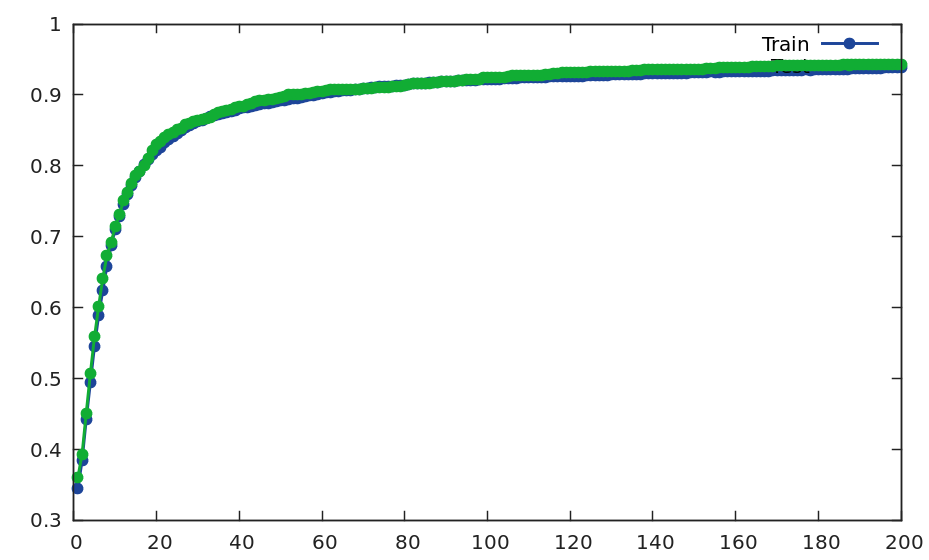
\includegraphics[scale=0.4]{Batch.png}


\section{Stochastic}

Temps mis: 71s\newline
Score Train : 0.966\newline
Score Test : 0.960\newline

Note : Optimum atteint en 3 itérations

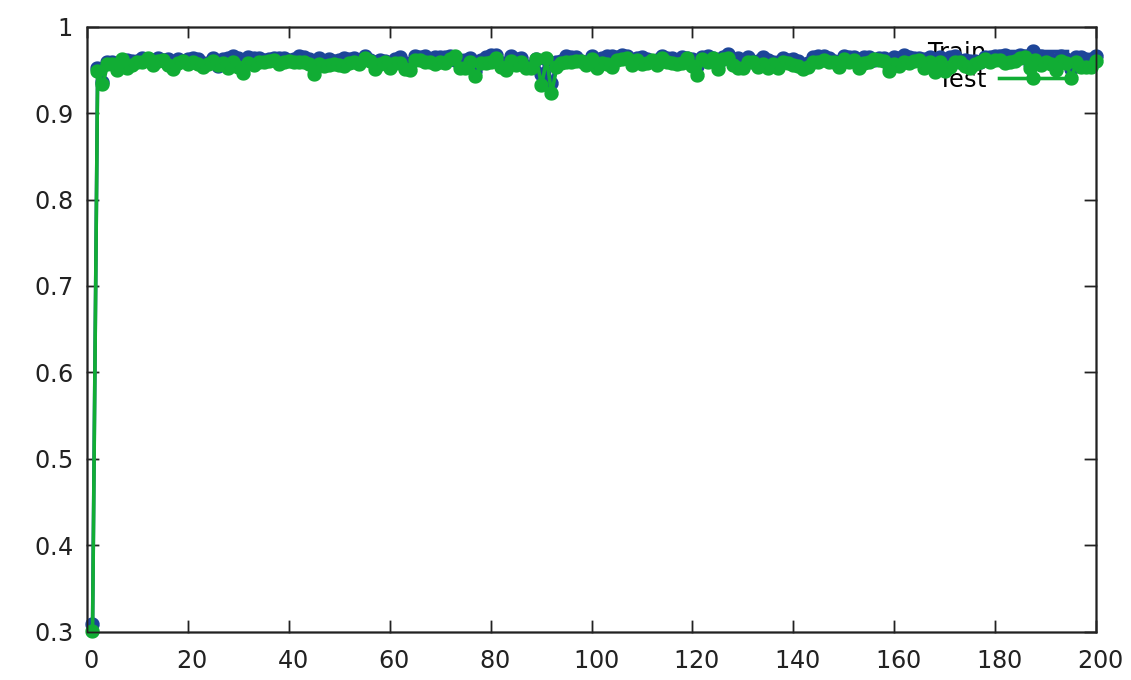
\includegraphics[scale=0.3]{Stoch.png}

\section{Mini-batch 10}

Temps mis : 69s\newline
Score Train : 0.966\newline
Score Test : 0.960\newline

Note : Optimum atteint en 10 itérations

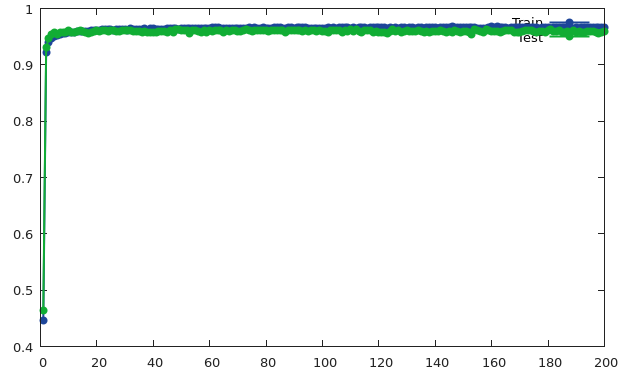
\includegraphics[scale=0.55]{Minibatch10.png}

\section{Mini-batch 100}

Temps mis: 19s\newline
Score Train : 0.962\newline
Score Test : 0.961\newline

Note : Optimum atteint en ~30 itérations

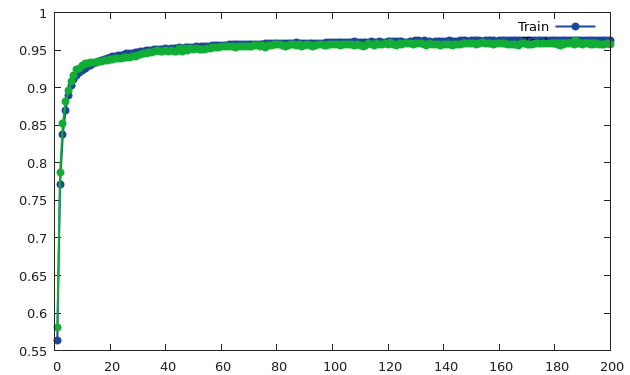
\includegraphics[scale=0.55]{Minibatch100.png}

\section{Conclusion des expés}

On constate que le batch met peu de temps à se calculer par rapport au stochastique (le batch est basé ssur des opérations matricielles, tandis que le stochastique, on itère sur tous les exemples un à un)

Par contre, il met énormément de temps à converger (à 200 itérations, il n'a pas complètement fini tandis que le stochastique converge en 3 itérations)

Le mini-batch est entre les deux, il est rapide en temps, et il converge bien plus rapidement que le batch.

Les performances en Train/Test sont extrêment corrélées, on ne constate pas de sur-apprentissage (Pas de baisse de la performance en test).


On peut noter aussi qu'il faut utiliser un learning rate plus petit pour le stochastique que pour le batch (C'est logique, car on veut faire des mises à jour plus importantes quand toute la base est prise en compte, et à l'inverse, de petites mises à jour pour un seul exemple)

\section{Split 90/10 : Classe positive :0 \newline Classe négative : Tous les autres}

Le temps de calcul est beaucoup plus long (pour 100 itérations cela prend environ 95 secondes avec le mini-batch) mais on obtient des scores légèrement supérieurs (0.98-0.99)

Le batch arrive quasiment à convergence, tandis que stochastique et mini-batch convergent en quelques itérations.


\begin{figure}
  \centering
  \textbf{Mini-Batch pour split 90/10}\par\medskip
  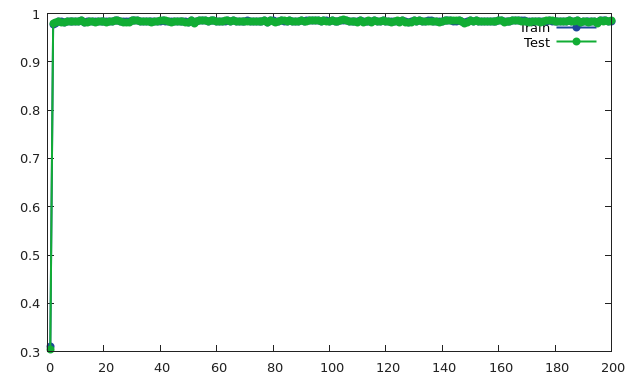
\includegraphics[scale=0.55]{splitMiniBatch90.png}
\end{figure}


\begin{figure}
  \centering
  \textbf{Batch pour split 90/10}\par\medskip
  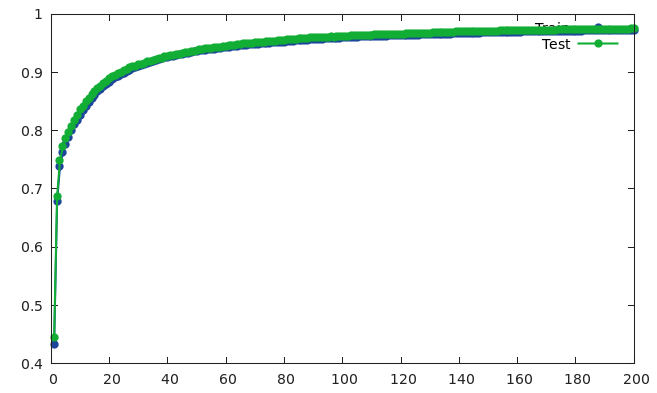
\includegraphics[scale=0.55]{splitBatch90.png}
\end{figure}


\subsection{Temps de calcul}

Le temps de calcul du gradient pour 200 itérations est exactement le même quelque soit le split.
\begin{enumerate}
\item 160s pour le batch
\item 190s pour le mini batch
\item s pour le stochastic
\end{enumerate}



\section{Split 50/50 : Classe positive :0,1,2,3,4 \newline Classe négative : 5,6,7,8,9}


Du au fait que l'on augmente la variance au sein d'une classe, les scores sont moins bons. En Train/Test, on obtient un score de 0.85 au maximum.\newline
Avec mini-batch et stochastique, cet optimum est atteint relativement rapidement (quelques itérations pour le stochastique, quelques dizaines pour le mini-batch).\newline
Avec le batch, 200 itérations ne suffisent pas à atteindre l'optimum (on arrive autour de 0.80)



\begin{figure}
  \centering
  \textbf{Batch pour split 50/50}\par\medskip
  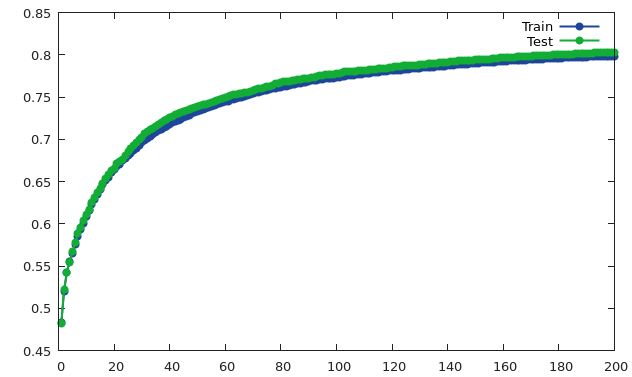
\includegraphics[scale=0.55]{splitBatch50.png}
\end{figure}

\begin{figure}
  \centering
  \textbf{MiniBatch pour split 50/50}\par\medskip
  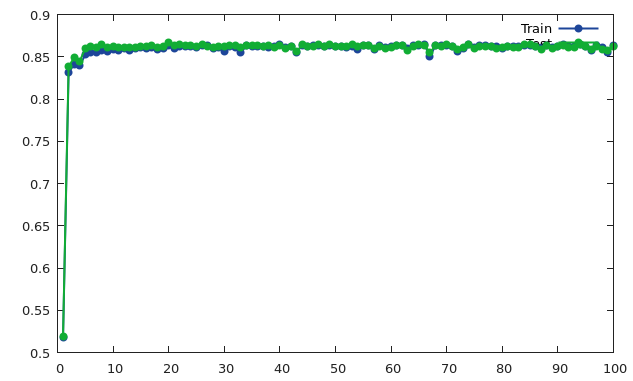
\includegraphics[scale=0.55]{splitMiniBatch50.png}
\end{figure}


\section{Critère Custom}

Avec le critère du Huber, on arrive à des résultats légèrement supérieur à un MSE (0.98 pour le MSE contre 0.99 pour le Huber), cela peut s'expliquer par le fait que le Huber est conçu pour de la classification tandis que le MSE est conçu pour de la régression.

Attention : Du à l'implémentation, Huber doit être utilisé avec un stochastique et non un batch.
\end{document}
